\documentclass[12pt,a4paper]{article}
\usepackage[utf8]{inputenc}
\usepackage[spanish,es-tabla]{babel}
\usepackage{geometry}
\usepackage{graphicx}
\usepackage{multirow}
\usepackage{tabularx}
\usepackage{mathptmx}
\usepackage{fancyhdr}
\usepackage{array}
\usepackage[table]{xcolor}
\usepackage{titlesec}
\usepackage{setspace}
\usepackage{microtype}
\usepackage{lastpage}
\usepackage{booktabs}
\usepackage{enumitem}
\usepackage{amsmath}
\usepackage{amsfonts}
\usepackage{amssymb}
\usepackage{listings}

\lstset{
  basicstyle=\ttfamily\footnotesize,
  backgroundcolor=\color{gray!10},
  frame=single,
  breaklines=true,
  tabsize=2,
  showstringspaces=false
}

\graphicspath{{images/}{../images/}{./}}

\geometry{
    top=4.7cm,
    bottom=2.5cm,
    left=2.5cm,
    right=2.5cm,
    headheight=3.9cm,
    headsep=0.4cm
}

\setstretch{1.15}
\setlength{\parindent}{0pt}
\setlength{\parskip}{0.45em}
\setlength{\tabcolsep}{4pt}

\titleformat{\section}
  {\normalfont\fontsize{12}{14.5}\bfseries}{\thesection.}{0.6em}{\uppercase}
\titlespacing*{\section}
  {0pt}{1.8ex plus 0.4ex minus 0.2ex}{0.6ex plus 0.2ex}

\titleformat{\subsection}
  {\normalfont\fontsize{11.5}{13.5}\bfseries}{\thesubsection.}{0.5em}{}
\titlespacing*{\subsection}
  {0pt}{1.4ex plus 0.3ex minus 0.1ex}{0.4ex plus 0.1ex}

\titleformat{\subsubsection}
  {\normalfont\fontsize{10.5}{12.5}\bfseries\itshape}{\thesubsubsection.}{0.4em}{}
\titlespacing*{\subsubsection}
  {0pt}{1.1ex plus 0.2ex minus 0.1ex}{0.3ex plus 0.1ex}

\newcolumntype{Y}{>{\centering\arraybackslash}X}
\newcolumntype{L}{>{\raggedright\arraybackslash}X}
\newcolumntype{C}{>{\centering\arraybackslash}X}

\definecolor{headerred}{RGB}{180, 0, 0}
\definecolor{darkred}{RGB}{140, 0, 0}
\definecolor{lightgraybg}{RGB}{248, 248, 248}
\definecolor{tableheader}{RGB}{232, 238, 246}

\newcommand{\docCodigo}{TI-SIGE-ENT-S2-004}
\newcommand{\docVersion}{1.0}
\newcommand{\docProceso}{INGENIERÍA DE SOFTWARE / DISEÑO DE BASE DE DATOS}
\newcommand{\docElaboracion}{02/09/2026}
\newcommand{\docRevision}{PENDIENTE DE REVISIÓN}
\newcommand{\docTitulo}{DISEÑO DE BASE DE DATOS RELACIONAL: MODELO ENTIDAD-RELACIÓN Y ESQUEMA LÓGICO POSTGRESQL}
\newcommand{\docOrganizacion}{FACULTAD DE INGENIERÍA EN SISTEMAS, ELECTRÓNICA E INDUSTRIAL}
\newcommand{\docSubOrganizacion}{CARRERA DE INGENIERÍA DE SOFTWARE}

\newcommand{\encabezadofrecuente}{%
    \renewcommand{\arraystretch}{1.15}%
    \noindent\makebox[\textwidth][c]{%
    \begin{tabularx}{\textwidth}{|>{\centering\arraybackslash}m{2.8cm}|Y|>{\centering\arraybackslash}m{4.8cm}|}
        \hline
        \multirow{4}{2.8cm}{\centering\raisebox{-1.15cm}{
\includegraphics[width=2.5cm,height=2.0cm,keepaspectratio]{images/logo.png}}}
        & \textbf{\fontsize{9}{11}\selectfont \docOrganizacion} 
        & \textbf{\fontsize{8}{10}\selectfont CÓDIGO:} \fontsize{8}{10}\selectfont \docCodigo \\
        \cline{3-3}
        & \textbf{\fontsize{8.5}{10.5}\selectfont \docSubOrganizacion} 
        & \textbf{\fontsize{8}{10}\selectfont VERSIÓN:} \fontsize{8}{10}\selectfont \docVersion \\
        \cline{2-3}
        & \textbf{\fontsize{8}{10}\selectfont PROCESO:} \fontsize{8}{10}\selectfont \docProceso 
        & \textbf{\fontsize{8}{10}\selectfont ELABORACIÓN:} \fontsize{8}{10}\selectfont \docElaboracion \\
        \cline{2-3}
        & \textbf{\fontsize{8.5}{10.5}\selectfont \docTitulo} 
        & \textbf{\fontsize{8}{10}\selectfont ÚLTIMA REVISIÓN:} \fontsize{8}{10}\selectfont \textbf{\textcolor{darkred}{\docRevision}} \\
        \hline
    \end{tabularx}%
    }%
}

\pagestyle{fancy}
\fancyhf{}
\fancyhead[C]{\encabezadofrecuente}
\fancyfoot[C]{\fontsize{10}{12}\selectfont Página \thepage\ de \pageref{LastPage}}
\renewcommand{\headrulewidth}{0pt}

\begin{document}

\section{Título}
\textbf{Denominación del Entregable:} Modelo Conceptual ER, Esquema Lógico Relacional y Diccionario de Datos PostgreSQL 18 (EDT 2.4)



\section{Introducción}
El modelo de datos relacional del sistema \textbf{SIGE} ha sido diseñado para operar en \textbf{PostgreSQL (18)}, garantizando transaccionalidad ACID pura, normalización en Tercera Forma Normal (3FN), integridad referencial estricta, control de aperturas extemporáneas por el Administrador, soporte para solicitudes de modificación de planes en ejecución, trazabilidad del estado por actividad y el registro secuencial del circuito de firmas en cascada institucional (Docente Responsable $\rightarrow$ Coordinador de Área $\rightarrow$ Coordinador de Carrera).

\section{Objetivo}

\subsection{Objetivo General}
Diseñar y estructurar la base de datos relacional en PostgreSQL 18 para el sistema SIGE, asegurando integridad referencial, normalización en 3FN y trazabilidad auditada de cambios para la arquitectura modular de Node.js + Express (v5).

\subsection{Objetivos Específicos}
\begin{enumerate}[leftmargin=1.5em, itemsep=2pt, topsep=2pt]
    \item Construir el diagrama Entidad-Relación (ERD) con las 9 entidades del modelo de gestión de calidad.
    \item Elaborar el diccionario de datos exhaustivo para las tablas maestras y de detalle.
    \item Crear los índices de rendimiento y restricciones de unicidad para firmas en cascada y semáforos de actividades.
\end{enumerate}

\section{Alcance}

\subsection{Límites de Persistencia (In-Scope)}
\begin{itemize}[leftmargin=1.5em, itemsep=2pt]
    \item Tablas para documentos, actividades, evidencias, firmas en cascada, solicitudes de cambio, habilitaciones extemporáneas y auditoría.
\end{itemize}

\subsection{Exclusiones (Out-of-Scope)}
\begin{itemize}[leftmargin=1.5em, itemsep=2pt]
    \item Los archivos físicos (PDFs) no se almacenan como blobs en PostgreSQL, sino como objetos en MinIO con URI y SHA-256 en base de datos.
\end{itemize}

\section{Definiciones}
\begin{itemize}[leftmargin=1.5em, itemsep=2pt]
    \item \textbf{3FN (Tercera Forma Normal):} Estado en el que no existen dependencias funcionales transitivas entre atributos no clave.
    \item \textbf{UUID v4:} Identificador único universal de 128 bits empleado como clave primaria no secuencial.
    \item \textbf{Índice Compuesto:} Estructura B-Tree sobre múltiples columnas para acelerar consultas complejas de ordenamiento o filtrado.
\end{itemize}

\section{Responsabilidades}
\begin{table}[htbp]
\centering
\small
\begin{tabularx}{\textwidth}{|>{\hsize=0.65\hsize\bfseries}X|>{\hsize=0.85\hsize}X|>{\hsize=1.5\hsize}X|}
    \hline
    \rowcolor{tableheader}
    Integrante & Rol en el Entregable & Responsabilidad Específica \\
    \hline
    Nixon Hurtado & Backend / DBA & Modelado ER, diseño de esquemas DDL, diccionario de datos y optimización de índices. \\
    \hline
    Steeven Toala & Líder / Arquitecto & Verificación de coherencia con las reglas de negocio y Clean Architecture. \\
    \hline
    Ing. Paulo Torres & Docente Tutor & Revisión y aprobación del modelo relacional institucional. \\
    \hline
\end{tabularx}
\caption{Matriz de Responsabilidades del Entregable EDT 2.4.}
\end{table}

\section{Normativa Legal y Técnica}
\begin{itemize}[leftmargin=1.5em, itemsep=2pt]
    \item \textbf{ANSI/ISO/IEC 9075:2023:} Database Language SQL standard.
    \item \textbf{ISO/IEC 27001:2022:} Control de integridad y almacenamiento seguro de datos.
\end{itemize}

\section{Método, Políticas y Contenidos}
El modelo ERD se normalizó en 3FN con claves foráneas protegidas ante borrados accidentales:

\begin{figure}[htbp]
    \centering
    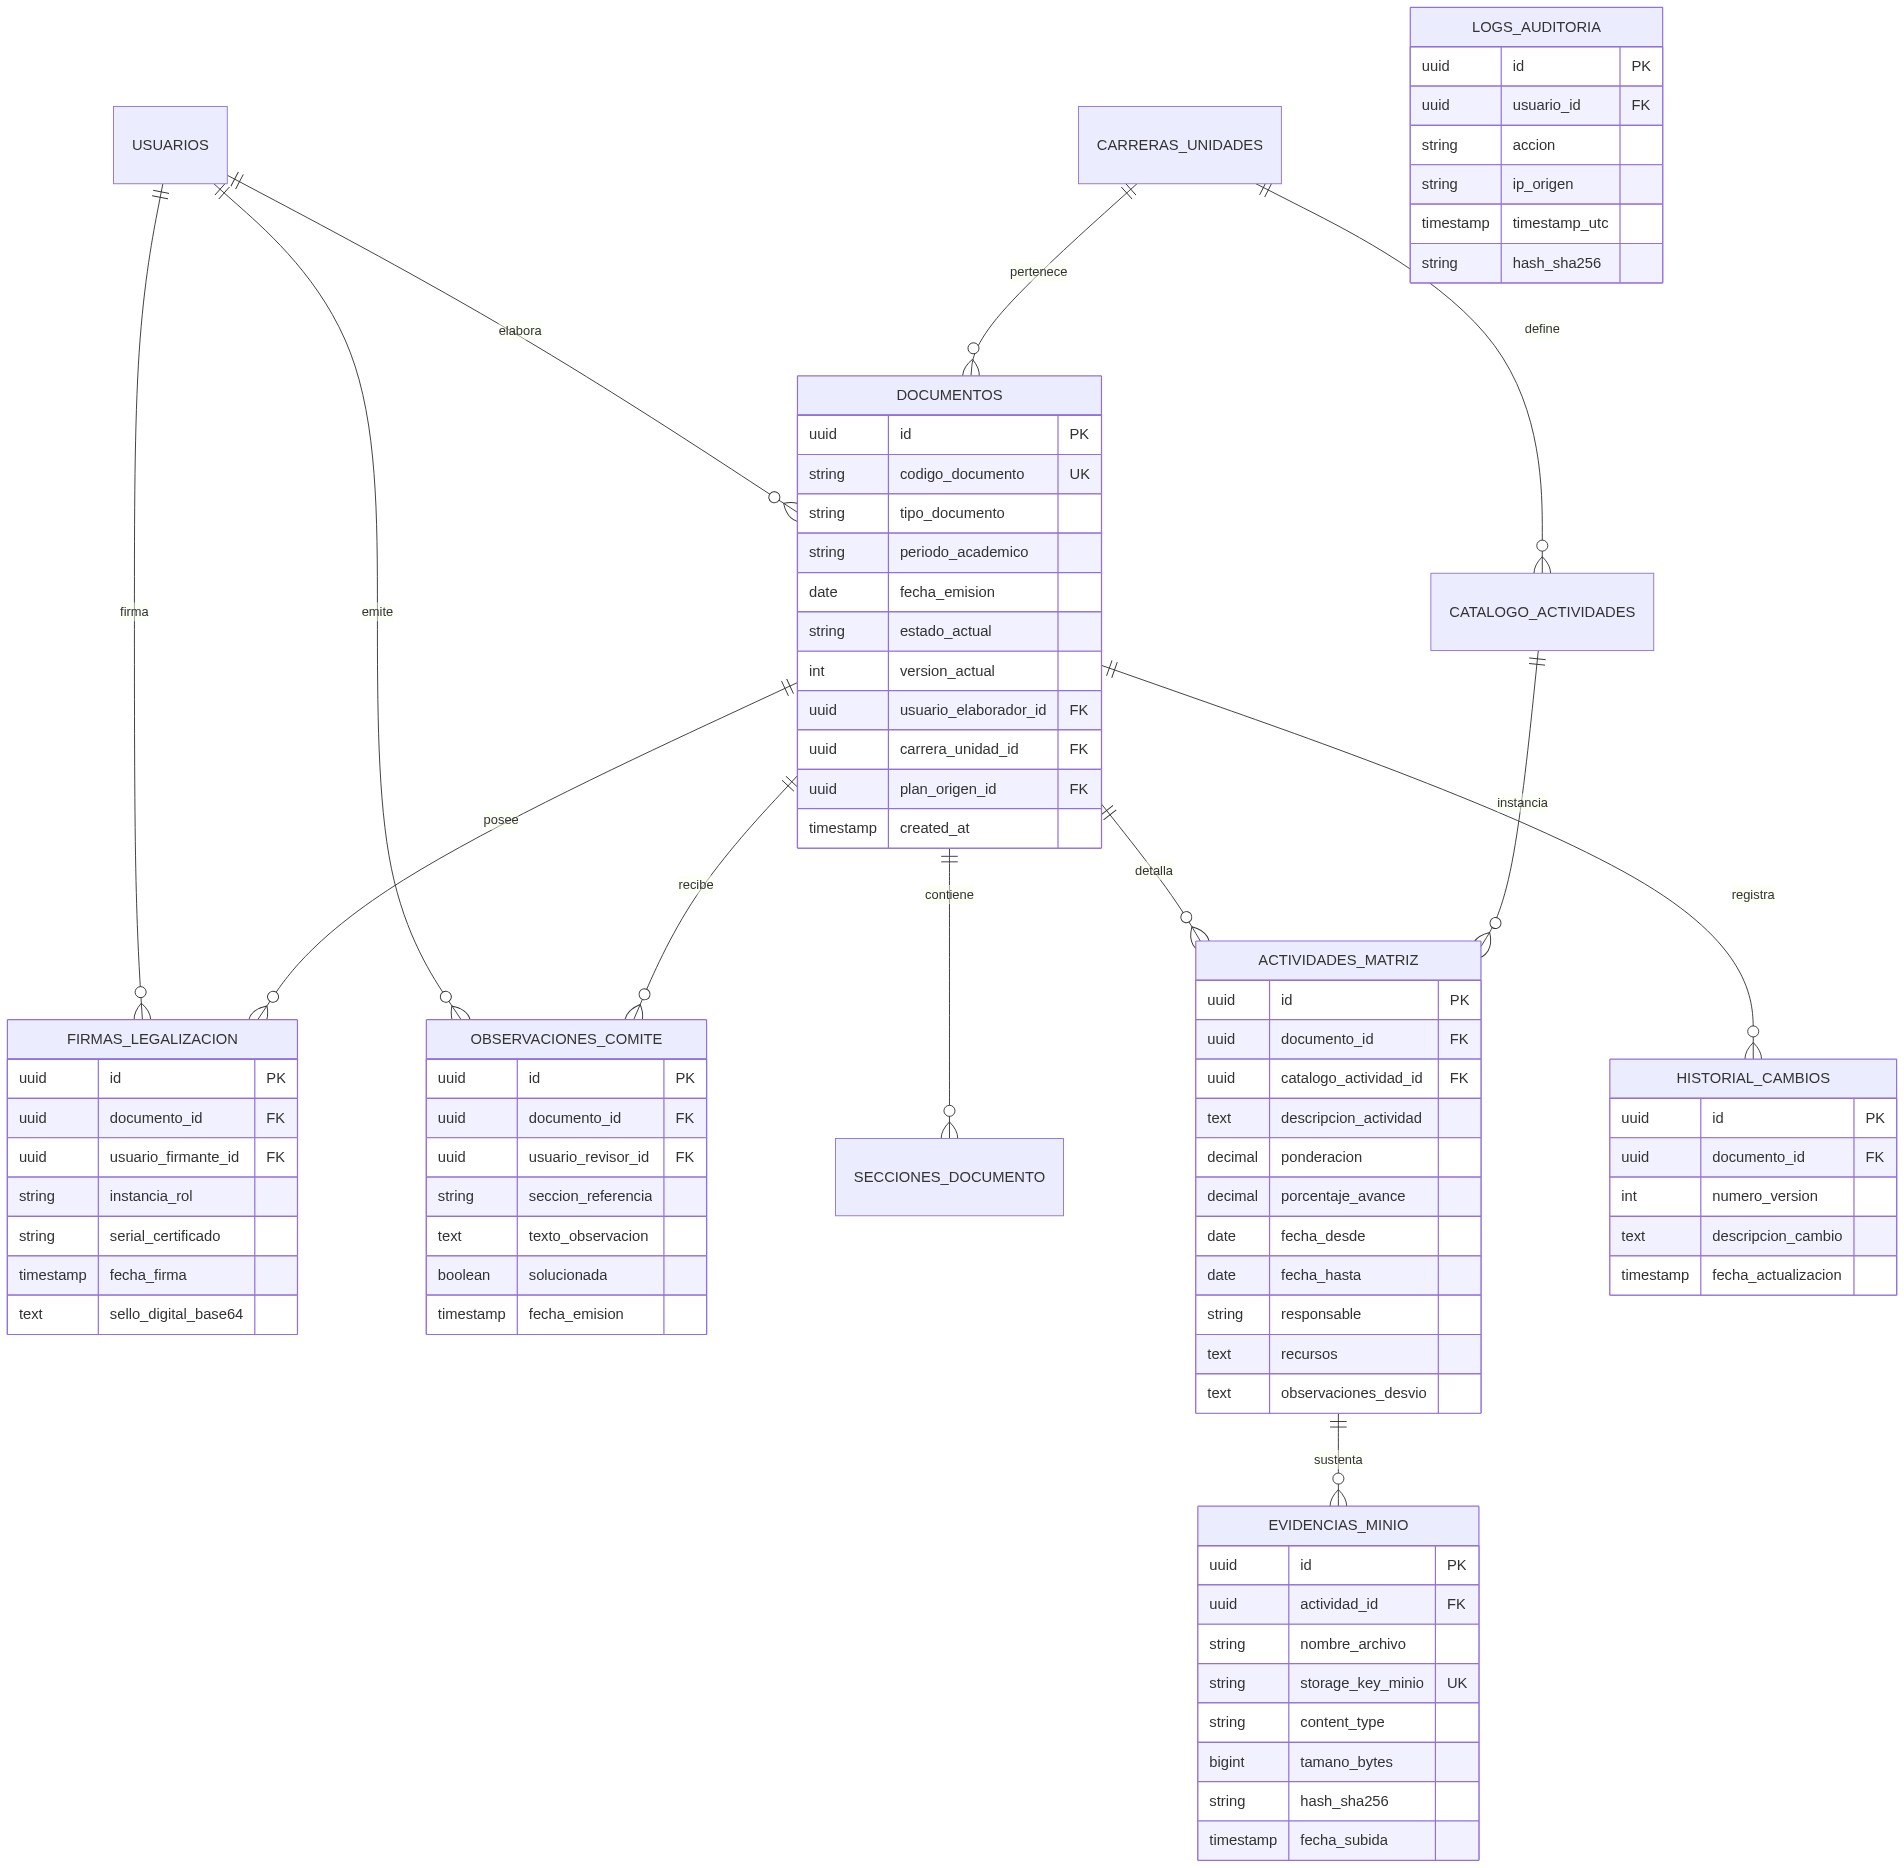
\includegraphics[width=0.85\textwidth,height=6.5cm,keepaspectratio]{images/s2_04_erd_postgresql.png}
    \caption{Diagrama Entidad-Relación (ERD) del Esquema Relacional en PostgreSQL 18.}
    \label{fig:s2_04_erd}
\end{figure}

\section{Descripción de actividades}

\subsection{Diccionario de Datos Lógico de Tablas Principales}

\subsection{Tabla: \texttt{DOCUMENTOS}}
Almacena el ciclo de vida de Planes de Trabajo e Informes de Cumplimiento.

\begin{table}[htbp]
\centering
\small
\begin{tabularx}{\textwidth}{|>{\hsize=0.65\hsize\bfseries}X|>{\hsize=0.5\hsize}X|>{\hsize=0.35\hsize\centering\arraybackslash}X|>{\hsize=1.5\hsize}X|}
    \hline
    \rowcolor{tableheader}
    Columna & Tipo & Nulable & Descripción y Restricciones \\
    \hline
    \texttt{id} & UUID & NO & PK, Identificador único universal (\texttt{gen\_random\_uuid()}). \\
    \hline
    \texttt{codigo\_documento} & VARCHAR(50) & NO & Código oficial único (ej. \texttt{SOFT-JD2026-INF-042-V01}). \\
    \hline
    \texttt{tipo\_documento} & VARCHAR(30) & NO & CHECK (\texttt{PLAN\_TRABAJO}, \texttt{INFORME\_CUMPLIMIENTO}). \\
    \hline
    \texttt{periodo\_academico} & VARCHAR(40) & NO & Período autodetectado (ej. \texttt{Julio 2026 -- Diciembre 2026}). \\
    \hline
    \texttt{fecha\_emision} & DATE & NO & Fecha autogenerada por el servidor (DEFAULT CURRENT\_DATE). \\
    \hline
    \texttt{estado\_actual} & VARCHAR(40) & NO & Máquina de estados (BORRADOR, EN\_EJECUCION, APROBADO, etc.). \\
    \hline
    \texttt{version\_actual} & INT & NO & Versión autoincremental (DEFAULT 1, CHECK $\ge 1$). \\
    \hline
    \texttt{usuario\_elaborador\_id} & UUID & NO & FK hacia \texttt{USUARIOS(id)} (Docente que elaboró el documento). \\
    \hline
    \texttt{carrera\_unidad\_id} & UUID & NO & FK hacia \texttt{CARRERAS\_UNIDADES(id)} (Pertenencia académica). \\
    \hline
\end{tabularx}
\caption{Diccionario de Datos de la Tabla \texttt{DOCUMENTOS}.}
\label{tab:s2_04_doc}
\end{table}

\subsection{Tabla: \texttt{HABILITACIONES\_EXTEMPORANEAS}}
Registra las prórrogas autorizadas por el Administrador ante retrasos en la planificación.

\begin{table}[htbp]
\centering
\small
\begin{tabularx}{\textwidth}{|>{\hsize=0.75\hsize\bfseries}X|>{\hsize=0.55\hsize}X|>{\hsize=0.3\hsize\centering\arraybackslash}X|>{\hsize=1.4\hsize}X|}
    \hline
    \rowcolor{tableheader}
    Columna & Tipo & Nulable & Descripción y Restricciones \\
    \hline
    \texttt{id} & UUID & NO & PK, Identificador único de la habilitación. \\
    \hline
    \texttt{documento\_id} & UUID & NO & FK hacia \texttt{DOCUMENTOS(id)} (Plan habilitado extemporáneo). \\
    \hline
    \texttt{admin\_id} & UUID & NO & FK hacia \texttt{USUARIOS(id)} (Administrador que autorizó). \\
    \hline
    \texttt{fecha\_otorgamiento} & TIMESTAMP & NO & Momento exacto de concesión (DEFAULT CURRENT\_TIMESTAMP). \\
    \hline
    \texttt{fecha\_limite\_gracia} & TIMESTAMP & NO & Límite temporal de vencimiento automático. \\
    \hline
    \texttt{motivo\_justificacion} & TEXT & NO & Sustento oficial de la apertura extemporánea. \\
    \hline
    \texttt{numero\_oficio\_respaldo} & VARCHAR(100) & NO & Código del memorando u oficio de soporte. \\
    \hline
\end{tabularx}
\caption{Diccionario de Datos de la Tabla \texttt{HABILITACIONES\_EXTEMPORANEAS}.}
\label{tab:s2_04_hab}
\end{table}

\subsection{Tabla: \texttt{ACTIVIDADES\_MATRIZ}}
Almacena las actividades con control de fechas \texttt{Desde} y \texttt{Hasta}, y estado granular por actividad.

\begin{table}[htbp]
\centering
\small
\begin{tabularx}{\textwidth}{|>{\hsize=0.7\hsize\bfseries}X|>{\hsize=0.55\hsize}X|>{\hsize=0.3\hsize\centering\arraybackslash}X|>{\hsize=1.45\hsize}X|}
    \hline
    \rowcolor{tableheader}
    Columna & Tipo & Nulable & Descripción y Restricciones \\
    \hline
    \texttt{id} & UUID & NO & PK, Identificador de la actividad. \\
    \hline
    \texttt{documento\_id} & UUID & NO & FK hacia \texttt{DOCUMENTOS(id)} ON DELETE CASCADE. \\
    \hline
    \texttt{descripcion\_actividad} & TEXT & NO & Detalle de la actividad planificada. \\
    \hline
    \texttt{ponderacion} & NUMERIC(5,2) & NO & Ponderación porcentual asignada ($0.00$ a $100.00$). \\
    \hline
    \texttt{porcentaje\_avance} & NUMERIC(5,2) & NO & Porcentaje real alcanzado ($0.00$ a $100.00$). \\
    \hline
    \texttt{fecha\_desde} & DATE & NO & Inicio programado de la actividad. \\
    \hline
    \texttt{fecha\_hasta} & DATE & NO & Fin programado (CHECK \texttt{fecha\_hasta >= fecha\_desde}). \\
    \hline
    \texttt{estado\_actividad} & VARCHAR(25) & NO & Enum (\texttt{PENDIENTE}, \texttt{EN\_EJECUCION}, \texttt{FINALIZADA}). \\
    \hline
    \texttt{responsable} & VARCHAR(150) & SI & Docente responsable asignado. \\
    \hline
    \texttt{recursos} & TEXT & SI & Recursos humanos, tecnológicos y materiales requeridos. \\
    \hline
    \texttt{medios\_verificacion} & TEXT & SI & Tipo de evidencia exigida (actas, oficios, etc.). \\
    \hline
    \texttt{observaciones\_desvio} & TEXT & SI & Justificación obligatoria si avance $< 100\%$. \\
    \hline
\end{tabularx}
\caption{Diccionario de Datos de la Tabla \texttt{ACTIVIDADES\_MATRIZ}.}
\label{tab:s2_04_act}
\end{table}

\subsection{Tabla: \texttt{FIRMAS\_LEGALIZACION}}
Controla el orden jerárquico estricto en cascada oficial de la FISEI:
\[
\text{1: Docente Responsable} \longrightarrow \text{2: Coordinador de Área} \longrightarrow \text{3: Coordinador de Carrera}
\]

\begin{table}[htbp]
\centering
\small
\begin{tabularx}{\textwidth}{|>{\hsize=0.7\hsize\bfseries}X|>{\hsize=0.55\hsize}X|>{\hsize=0.3\hsize\centering\arraybackslash}X|>{\hsize=1.45\hsize}X|}
    \hline
    \rowcolor{tableheader}
    Columna & Tipo & Nulable & Descripción y Restricciones \\
    \hline
    \texttt{id} & UUID & NO & PK, Identificador de la firma legalizada. \\
    \hline
    \texttt{documento\_id} & UUID & NO & FK hacia \texttt{DOCUMENTOS(id)}. \\
    \hline
    \texttt{usuario\_firmante\_id} & UUID & NO & FK hacia \texttt{USUARIOS(id)} (Firmante acreditado). \\
    \hline
    \texttt{fase\_documento} & VARCHAR(30) & NO & CHECK (\texttt{PLANIFICACION\_INICIAL}, \texttt{INFORME\_FINAL}). \\
    \hline
    \texttt{orden\_cascada} & INT & NO & \textbf{Posición jerárquica estricta (1, 2 o 3)}. \\
    \hline
    \texttt{rol\_instancia} & VARCHAR(40) & NO & CHECK (\texttt{DOCENTE}, \texttt{COORD\_AREA}, \texttt{COORD\_CARRERA}). \\
    \hline
    \texttt{estado\_firma} & VARCHAR(20) & NO & CHECK (\texttt{PENDIENTE}, \texttt{FIRMADO}, \texttt{RECHAZADO}). \\
    \hline
    \texttt{serial\_certificado} & VARCHAR(150) & SI & Número de serie del certificado digital .p12 (FirmaEC). \\
    \hline
    \texttt{fecha\_firma} & TIMESTAMP & SI & Timestamp exacto en el que se estampó la firma. \\
    \hline
    \texttt{sello\_digital\_base64} & TEXT & SI & Sello criptográfico generado por FirmaEC. \\
    \hline
\end{tabularx}
\caption{Diccionario de Datos de la Tabla \texttt{FIRMAS\_LEGALIZACION}.}
\label{tab:s2_04_firmas}
\end{table}

\subsection{Índices de Rendimiento y Control de Integridad DDL}
\begin{lstlisting}[language=SQL]
-- Indice unico: Garantiza que no existan firmas duplicadas en el mismo orden de cascada
CREATE UNIQUE INDEX uq_firmas_documento_fase_orden 
ON FIRMAS_LEGALIZACION(documento_id, fase_documento, orden_cascada);

-- Indice para verificar rapidamente que firma es la siguiente en la cascada
CREATE INDEX idx_firmas_cascada_estado 
ON FIRMAS_LEGALIZACION(documento_id, orden_cascada, estado_firma);

-- Indice para verificar prorrogas activas otorgadas por el Administrador
CREATE INDEX idx_habilitaciones_documento_vigencia 
ON HABILITACIONES_EXTEMPORANEAS(documento_id, fecha_limite_gracia);

-- Indice para consultar solicitudes de reprogramacion de planes
CREATE INDEX idx_solicitudes_plan_estado 
ON SOLICITUDES_MODIFICACION_PLAN(plan_trabajo_id, estado_solicitud);

-- Indices para monitoreo y semaforos de actividades por fechas Desde-Hasta
CREATE INDEX idx_actividades_fechas_estado 
ON ACTIVIDADES_MATRIZ(documento_id, fecha_hasta, estado_actividad);

-- Indice para evidencias de soporte en MinIO
CREATE INDEX idx_evidencias_actividad_id 
ON EVIDENCIAS_MINIO(actividad_id);
\end{lstlisting}

\vspace{0.3cm}

% =============================================================
% FIRMAS DE RESPONSABILIDAD
% =============================================================
\section{Firmas de Responsabilidad}

\noindent
\renewcommand{\arraystretch}{1.2}
\begin{tabularx}{\textwidth}{|>{\raggedright\arraybackslash}m{2.9cm}|>{\raggedright\arraybackslash}X|>{\centering\arraybackslash}m{4.6cm}|>{\centering\arraybackslash}m{2.3cm}|}
    \hline
    \rowcolor{headerred}
    \textcolor{white}{\textbf{ACCIÓN}} & \textcolor{white}{\textbf{NOMBRE Y CARGO}} & \textcolor{white}{\textbf{FIRMA}} & \textcolor{white}{\textbf{FECHA}} \\
    \hline
    \textbf{Elaborado por:} & Nixon Hurtado\newline \textit{Desarrollador Backend / Ingeniero DBA} & \parbox[c]{4.4cm}{\centering\vspace{4pt}
\includegraphics[height=1.5cm,width=4.0cm,keepaspectratio]{images/firma_heidi.png}\vspace{4pt}} & 02/09/2026 \\
    \hline
    \textbf{Revisado por:} & Steeven Toala\newline \textit{Líder de Proyecto / Arquitecto Software} & \parbox[c]{4.4cm}{\centering\vspace{10pt}\textbf{\textcolor{gray!80}{\scriptsize [ PENDIENTE DE REVISIÓN ]}}\vspace{10pt}} & \textbf{\textcolor{gray!90}{Pendiente}} \\
    \hline
    \textbf{Aprobado por:} & Ing. Paulo Torres\newline \textit{Docente Tutor - Gestión Proyectos Software} & \parbox[c]{4.4cm}{\centering\vspace{10pt}\textbf{\textcolor{gray!80}{\scriptsize [ PENDIENTE DE APROBACIÓN ]}}\vspace{10pt}} & \textbf{\textcolor{gray!90}{Pendiente}} \\
    \hline
\end{tabularx}

\vspace{0.4cm}

% =============================================================
% CONTROL DE CAMBIOS
% =============================================================
\section{Control de Cambios}

\noindent
\renewcommand{\arraystretch}{1.2}
\begin{tabularx}{\textwidth}{|>{\hsize=0.45\hsize\centering\arraybackslash}X|>{\hsize=1.55\hsize\raggedright\arraybackslash}X|>{\hsize=1.2\hsize\raggedright\arraybackslash}X|>{\hsize=0.8\hsize\centering\arraybackslash}X|}
    \hline
    \rowcolor{gray!20}
    \textbf{Versión} & \textbf{Descripción del cambio} & \textbf{Responsable del cambio} & \textbf{Fecha de aprobación} \\
    \hline
    1.0 & Diseño de base de datos relacional ERD, diccionario de datos y DDL PostgreSQL 18 / Pendiente de revisión & Nixon Hurtado & \textbf{\textcolor{gray!90}{Pendiente de Revisión}} \\
    \hline
\end{tabularx}

\vspace{0.4cm}

\section{Anexos}
\subsection*{Anexo 1: Scripts DDL de Inicialización PostgreSQL 18 y Pool de Conexiones}
Estructura de \texttt{backend/src/database/schema.sql}, \texttt{seed.sql} y \texttt{init.js} para la inicialización determinista de la base de datos relacional y configuración del pool con la librería \texttt{pg}.

\end{document}
